% =============================================================================
% 5. DEMOSTRACION
% =============================================================================
\section{Demostraci\'on}
\label{sec:demo}

\subsection{C\'omo ejecutar el servicio}

El profesor puede levantar el servicio con un \'unico comando:

\begin{lstlisting}[language=bash, caption={Comando para ejecutar el servicio.}]
docker run --rm -p 8000:8000 ghcr.io/ahincho/chest-xpert-backend:latest
\end{lstlisting}

\noindent
Log esperado al arrancar:

\begin{lstlisting}[language={}, caption={Logs de arranque del servicio.}]
INFO: Loading ONNX model from models/chest-xpert-model.onnx
INFO: ONNX model loaded successfully
INFO: FilterService initialized with threshold=5.0
INFO: Uvicorn running on http://0.0.0.0:8000
\end{lstlisting}

\subsection{Ejemplo de solicitud}

Una vez arrancado, se puede enviar una radiograf\'ia al endpoint \texttt{/predict}:

\begin{lstlisting}[language=bash, caption={Request de ejemplo con curl.}]
curl -X POST http://localhost:8000/predict \
  -F "file=@radiografia_torax.png"
\end{lstlisting}

\subsection{Respuesta del modelo}

\begin{lstlisting}[language={}, caption={Response JSON real del servicio.}]
{
  "success": true,
  "predictions": [
    {"pathology": "Cardiomegaly",    "probability": 0.2543},
    {"pathology": "Edema",           "probability": 0.1606},
    {"pathology": "Consolidation",   "probability": 0.0134},
    {"pathology": "Atelectasis",     "probability": 0.0740},
    {"pathology": "Pleural Effusion","probability": 0.0610}
  ]
}
\end{lstlisting}

\subsection{Interpretaci\'on de resultados}

Cada valor en \texttt{predictions} es la probabilidad independiente ($\in [0, 1]$) de que la patolog\'ia est\'e presente en la radiograf\'ia. El modelo realiza clasificaci\'on multi-etiqueta, lo que significa que m\'ultiples patolog\'ias pueden estar presentes simult\'aneamente.

\begin{itemize}
    \item Valores $> 0.5$: alta sospecha de la patolog\'ia.
    \item Valores $\in [0.2, 0.5]$: sospecha moderada, requiere revisi\'on.
    \item Valores $< 0.2$: baja probabilidad.
\end{itemize}

El modelo est\'a dise\~nado como herramienta de \textbf{triaje}, no como diagn\'ostico definitivo. Debe utilizarse siempre bajo supervisi\'on de un profesional de salud.

\begin{figure}[H]
    \centering
    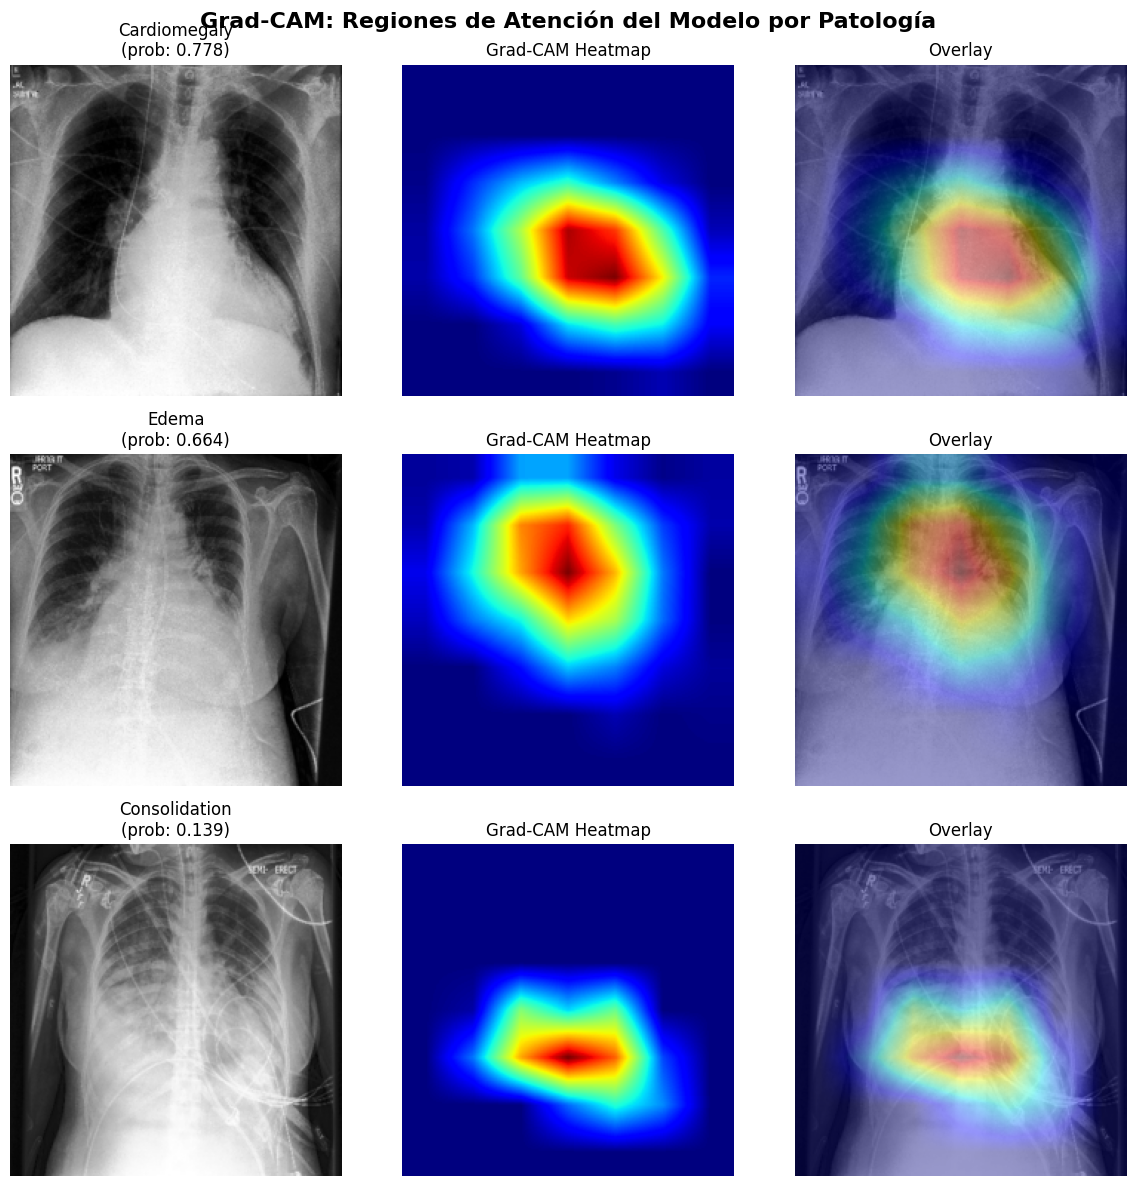
\includegraphics[width=0.85\textwidth]{figures/gradcam-cardiomegaly-edema-consolidation.png}
    \caption{Mapas Grad-CAM del modelo: Cardiomegaly (silueta card\'iaca), Edema (campos pulmonares) y Consolidation (opacidad focal). Atenci\'on anat\'omicamente correcta.}
    \label{fig:gradcam}
\end{figure}

\subsection{Respuestas de error}

El servicio maneja gracefully los errores:

\begin{itemize}
    \item \textbf{Imagen a color} (no radiograf\'ia): filtro RGB-Diff rechaza con mensaje descriptivo.
    \item \textbf{Archivo corrupto}: error 400 con mensaje ``Cannot decode image''.
    \item \textbf{Archivo demasiado grande} ($>$10MB): error 413.
    \item \textbf{Campo faltante}: error 422 con validaci\'on Pydantic.
\end{itemize}
